\documentclass{techrep}
%%%%%%%%%%%%%%%%%%%%%%%%%%%%%%%%%%%%%%%%%%%%%%%%%%%%%
%
%  Definition Starts
%
%%%%%%%%%%%%%%%%%%%%%%%%%%%%%%%%%%%%%%%%%%%%%%%%%%%%%

\usepackage{amsfonts}
\usepackage{amsthm}

\newcommand{\centeripe}[1]{\begin{center}\Ipe{#1}\end{center}}
\newcommand{\comment}[1]{}

\newcommand{\centerpsfig}[1]{\centerline{\psfig{#1}}}

\newcommand{\seclabel}[1]{\label{sec:#1}}
\newcommand{\Secref}[1]{Section~\ref{sec:#1}}
\newcommand{\secref}[1]{\mbox{Section~\ref{sec:#1}}}

\newcommand{\alglabel}[1]{\label{alg:#1}}
\newcommand{\Algref}[1]{Algorithm~\ref{alg:#1}}
\newcommand{\algref}[1]{\mbox{Algorithm~\ref{alg:#1}}}

\newcommand{\applabel}[1]{\label{app:#1}}
\newcommand{\Appref}[1]{Appendix~\ref{app:#1}}
\newcommand{\appref}[1]{\mbox{Appendix~\ref{app:#1}}}

\newcommand{\tablabel}[1]{\label{tab:#1}}
\newcommand{\Tabref}[1]{Table~\ref{tab:#1}}
\newcommand{\tabref}[1]{Table~\ref{tab:#1}}

\newcommand{\figlabel}[1]{\label{fig:#1}}
\newcommand{\Figref}[1]{Figure~\ref{fig:#1}}
\newcommand{\figref}[1]{\mbox{Figure~\ref{fig:#1}}}

\newcommand{\eqlabel}[1]{\label{eq:#1}}
%\renewcommand{\eqref}[1]{(\ref{eq:#1})}
\newcommand{\myeqref}[1]{(\ref{eq:#1})}
\newcommand{\Eqref}[1]{Equation~(\ref{eq:#1})}

\newtheorem{theorem}{Theorem}{\bfseries}{\itshape}
\newcommand{\thmlabel}[1]{\label{thm:#1}}
\newcommand{\thmref}[1]{Theorem~\ref{thm:#1}}

\newtheorem{lemma}{Lemma}{\bfseries}{\itshape}
\newcommand{\lemlabel}[1]{\label{lem:#1}}
\newcommand{\lemref}[1]{Lemma~\ref{lem:#1}}

\newtheorem{conj}{Conjecture}{\bfseries}{\itshape}
\newcommand{\conjlabel}[1]{\label{lem:#1}}
\newcommand{\conjref}[1]{Conjecture~\ref{lem:#1}}

\newtheorem{corollary}{Corollary}{\bfseries}{\itshape}
\newcommand{\corlabel}[1]{\label{cor:#1}}
\newcommand{\corref}[1]{Corollary~\ref{cor:#1}}

\newtheorem{obs}{Observation}{\bfseries}{\itshape}
\newcommand{\obslabel}[1]{\label{obs:#1}}
\newcommand{\obsref}[1]{Observation~\ref{obs:#1}}

\newtheorem{clm}{Claim}{\bfseries}{\itshape}
\newcommand{\clmlabel}[1]{\label{clm:#1}}
\newcommand{\clmref}[1]{Claim~\ref{clm:#1}}

\newtheorem{assumption}{Assumption}{\bfseries}{\rm}
\newenvironment{ass}{\begin{assumption}\rm}{\end{assumption}}
\newcommand{\asslabel}[1]{\label{ass:#1}}
\newcommand{\assref}[1]{Assumption~\ref{ass:#1}}

\newcommand{\proclabel}[1]{\label{alg:#1}}
\newcommand{\procref}[1]{Procedure~\ref{alg:#1}}

\theoremstyle{definition}

\newtheorem{definition}{Definition}
\newcommand{\deflabel}[1]{\label{rem:#1}}
\newcommand{\defref}[1]{Definition~\ref{rem:#1}}


\newtheorem{rem}{Remark}
\newcommand{\remlabel}[1]{\label{rem:#1}}
\newcommand{\remref}[1]{Remark~\ref{rem:#1}}

\newtheorem{lesson}{Lesson}
\newcommand{\leslabel}[1]{\label{les:#1}}
\newcommand{\lesref}[1]{Lesson~\ref{les:#1}}

\newtheorem{op}{Open Problem}
\newcommand{\oplabel}[1]{\label{op:#1}}
\newcommand{\opref}[1]{Open Problem~\ref{op:#1}}
\newtheorem{prb}{Problem}{\bfseries}{\rm}

\theoremstyle{plain}

\newcommand{\etal}{et al.}

\newcommand{\keywords}[1]{\noindent\textbf{Keywords:} #1}
\newcommand{\voronoi}{Vorono\u\i}
\newcommand{\ceil}[1]{{\lceil #1 \rceil}}
\newcommand{\Ceil}[1]{{\left\lceil #1 \right\rceil}}
\newcommand{\floor}[1]{{\lfloor #1 \rfloor}}
\newcommand{\Floor}[1]{{\left\lfloor #1 \right\rfloor}}
\newcommand{\R}{\mathbb{R}}
\newcommand{\N}{\mathbb{N}}
\newcommand{\Z}{\mathbb{Z}}
\newcommand{\Sp}{\mathbb{S}}
\newcommand{\E}{\mathrm{E}}
\newcommand{\DD}{\ensuremath{\mathcal{D}}}


\usepackage{verbatim}
\usepackage{algorithm2e}
\usepackage[utf8]{inputenc}
\usepackage{microtype}
\usepackage{amsthm,amsmath,graphicx}
\usepackage{caption}
\usepackage{subcaption}
\usepackage[letterpaper]{hyperref}
\usepackage[table,dvipsnames]{xcolor}
\definecolor{linkblue}{named}{Blue}
\hypersetup{colorlinks=true, linkcolor=linkblue,  anchorcolor=linkblue,
	citecolor=linkblue, filecolor=linkblue, menucolor=linkblue,
	urlcolor=linkblue}
\setlength{\parskip}{1ex}
\usepackage{wasysym}
\usepackage{graphicx}
\usepackage{caption}
\usepackage{enumitem}
\usepackage{thmtools, thm-restate}
\usepackage{wrapfig}
%\usepackage{mathrsfs}
\usepackage{float}
\usepackage{stackrel}
\usepackage{fixfoot}
\usepackage[utf8]{inputenc}
\usepackage[english]{babel}
\usepackage{mathrsfs}
\usepackage{venturis}
\usepackage{placeins}

\listfiles

%\graphicspath{{./graphics/}}%helpful if your graphic files are in another directory

\newtheorem{thm}{Theorem}
\newtheorem{lem}[thm]{Lemma}

\newcommand{\notes}[1]{\marginpar{\tiny{#1}}}

\newlength\problemsep
\setlength\problemsep{10pt}
\newcommand{\given}{}
\newcommand{\find}{}
\newcommand{\nogo}{\textsc{impossible}}
\newcommand{\go}{\textsc{possible}}
%\newcommand{\bdry}[1]{\ensuremath{\textsl{bd}\  #1}}
\newcommand{\bdP}{\ensuremath{\partial P}}
%\newcommand{\bdPccw}[1]{\ensuremath{\bdP^{ccw}(#1)}}
\newcommand{\bdPccw}[1]{\ensuremath{\partial^{+}(#1)}}
\newcommand{\bdPcw}[1]{\ensuremath{\partial^{-}(#1)}}
\newcommand{\ERCW}[1]{\ensuremath{R_{\textsl{cw}}( #1 )}}
\newcommand{\ERCCW}[1]{\ensuremath{R_{\textsl{ccw}}( #1 )}}
%\newcommand{\ERSPLIT}[1]{\ensuremath{R_{\textsl{split}}( #1 )}}
\newcommand{\ERSPLIT}[1]{\ensuremath{S( #1 )}}
\newcommand{\vangle}[1]{\ensuremath{u_{#1}}}
\newcommand{\vanglecw}[1]{\ensuremath{u_{#1}^{\textsl{\tiny cw}}}}
\newcommand{\vangleccw}[1]{\ensuremath{u_{#1}^{\textsl{\tiny ccw}}}}
%\newcommand{\vangleccw}[1]{\ensuremath{w_{#1 (ccw)}}}
\newcommand{\accumccw}[1]{\ensuremath{\textsl{accum}^{\textsl{\tiny ccw}}(#1)}}
\newcommand{\accumcw}[1]{\ensuremath{\textsl{accum}^{\textsl{\tiny cw}}(#1)}}
\newcommand{\pifrac}[2]{\ensuremath{\frac{#1 \pi}{#2}}}
\newcommand{\piover}[1]{\pifrac{}{#1}}
\newcommand{\piovertwo}{\ensuremath{\frac{\pi}{2}}}
\newcommand{\threepiovertwo}{\ensuremath{\frac{3\pi}{2}}}
\newcommand{\tqpi}{\pifrac{3}{4}}
\newcommand{\sed}[1]{\ensuremath{D(#1)}}
\newcommand{\bd}[1]{\ensuremath{\partial D(#1)}}



\newenvironment{problem}[1] {			% the typesetting here needs work.
	\vspace{\problemsep}
	\noindent{\scshape \underline{#1}}
	\renewcommand\descriptionlabel[1]%
	{\hspace{\labelsep}\textsc{##1}}
	\renewcommand{\given}{\item[Given:]}
	\renewcommand{\find}{\item[Find:]}
	\begin{description}
	}{
	\end{description}
	\vspace{\problemsep}
}

%\newcommand{\jit}[1]{\textcolor{blue}{Jit: #1}}
\newcommand{\jit}[1]{}
\newcommand{\tom}[1]{\textcolor{teal}{Tom: #1}}

\bibliographystyle{abbrv}

%%%%%%%%%%%%%%%%%%%%%%%%%%%%%%%%%%%%%%%%%%%%%%%%%%%%%
%
%  Definitions over
%
%%%%%%%%%%%%%%%%%%%%%%%%%%%%%%%%%%%%%%%%%%%%%%%%%%%%%



\usepackage{graphicx} % Required for inserting images

\title{TFHE}
%\author{Navjeet Sandhu}
%\date{September 2024}

\begin{document}

	\maketitle

	\section{Introduction}
TFHE is a Fully Homomorphic Encryption (FHE) scheme. It is an encryption scheme that allows you to perform computations over encrypted data. 

 	\subsection{Integer ring modulo $\Z_{q}$}
	An integer ring modulo q (also called integers modulo a prime number), denoted by $\Z_{q}$, is a mathematical structure known as a cyclic group or finite field in abstract algebra. Specifically, it is the set of residue classes of integers modulo q. This means it's the set of all possible remainders when integers are divided by q. For example, if q equals 2, then $\Z_{q}$ (which is $\Z_{2}$ in this case) includes only 0 and 1 because any integer either leaves a remainder of 0 or 1 when divided by 2. In the field of cryptography, we typically work with finite fields. The exciting thing about working in a finite field is that the polynomial coefficients “wrap around” when multiplied. So, regardless of how much polynomial arithmetic we perform, the polynomial coefficients can still be bounded in a fixed range, which is very attractive from an implementation perspective. If q equals 17, then $\Z_{q}$ (which is $\Z_{17}$ in this case) includes only 0 to 16 because any integer leaves a remainder of 0 to 16 when divided by 17. Hence the vector multiplication for vectors $g = [1, 2, 3, 4]$, and $h = [5, 6, 7, 8]$ with modulo a prime number $q = 17$ is  $[5, 16, 0, 9, 10, 1, 15]$

	\subsection{Congruence}
	The symbol $\equiv$ denotes congruence and is different from equality. While equality means that items are the same, congruence means items have the same remainder when divided by mod. In a ring $\Z_{7681}$  and $n = 4$, the 4-th root of unity, which satisfy the condition $\omega^4 \equiv 1$ mod $7681$ are ${3383, 4298, 7680}$.



	\section{TFHE Ciphertexts}
 TFHE mainly uses three ciphertext types: LWE, RLWE, and RGSW. All of them have different properties which will be useful in the homomorphic operations

	\section{GLWE}
General LWE, or GLWE includes both of LWE, RLWE

\subsection{LWE}
LWE encryption supports encrypting small-bit-width integers by placing those bits in the most significant bits of a machine word—for simplicity, say it’s a 4-bit integer in the top-most bits of a 32-bit integer with all the other bits initialized to zero, and call that whole encoded plaintext. The secret key is a random binary vector of some fixed length chosen to achieve a specific security. Then, sample a random length vector of 32-bit integers to encrypt, take a dot product with the secret key, add the message, and add some random noise. The encrypted value is both the random samples chosen and the noise-masked result. LWE decryption then reverses this process: re-compute the dot product and subtract it from the output of the encryption. But at the end, you must apply a rounding step to remove the noise added to the ciphertext during encryption. Because the message is in the highest-order bits of the message (say, bits 28-31) and because the noise added was not very large, rounding to the nearest multiple removes it. 

\subsection{RLWE}
In RLWE, the scalar multiplications and additions from LWE are upgraded to polynomial multiplications and additions. We pick a polynomial degree as the maximum degree (say 1024), the coefficients are always integers modulo some chosen modulus q, and finally, we pick a polynomial, usually $x^n+1$, and represent the result of every operation as a remainder when divided by that polynomial. One or more small integer messages are encoded into a polynomial to encrypt. The secret key is a list of random polynomials with binary coefficients, and the samples are random polynomials with uniformly random mod q coefficients. Then, you take a dot product, add the message, and add a similar “noise polynomial” to mask the result. The main advantage of using RLWE over LWE is that you can pack many messages into a single polynomial and the homomorphic operations you apply to all the messages. 

	\subsection{LWE and RLWE from GLWE }
 When we instantiate GLWE with $k = n$ and $N = 1$, we get LWE. Observe that $ R_q$ is actually $ Z_q$ when $ N = 1$. We use small letters for (modular) integers (i.e., b, m, e ...).

 	\begin{align*}
		b &= \sum_{i=0}^{k-1}a_i . s_i + \bigtriangleup m + e \in \Z_{q}  \\
	\end{align*}

When we instantiate GLWE with $k = 1$, we get RLWE. Here, we use capital letters for polynomials. 

	\begin{align*}
		B &= A . S + \bigtriangleup M + E \in R_q  \\
	\end{align*}


	\subsection{Secret key}
To generate any ciphertext, we first need a secret key. With  GLWE ciphertexts, the secret key is a list of 
 random polynomials from R:

	\begin{align*}
		\overrightarrow{S} &= (S_0,S_1,...S_{k-1}) \in R^k
	\end{align*}

The coefficients of the elements can be sampled from a uniform binary distribution, a uniform ternary distribution, a Gaussian distribution, or a uniform distribution. Please note that we can find parameters to achieve the desired security level for these secret keys.

\subsubsection{Example}

Let’s choose N (degree or dimension) = 4 and k =2. Let's sample the secret key with a uniform binary distribution of a degree N — 1 polynomial. In this example, the secret keys are [0,1,1,0] and [1,0,1,1].



\begin{align*} 
\overrightarrow{S} &= ([0,1,1,0],[1,0,1,1]) \in R^2 \\ 
\overrightarrow{S} &= (0 + x + x^2 + 0x^3,1 + 0x + x^2 + x^3) \in R^2 \\ 
\overrightarrow{S} &= (x + x^2, 1 + x^2 + x^3) \in R^2 \\ 
\end{align*}

\subsubsection{Example TFHEpp lvl1param}
For TFHEpp lvl1param, the value for N = $1024$, k = $1$. The key value maximum is $1$, and the minimum is $-1$. For example:

\begin{align*} 
\overrightarrow{S} &= ([0, 1, 0, -1, -1 ..... 1]) \in R^1 \\ 
\overrightarrow{S} &= (x - x^3 - x^5 - x^6 .... + x^{1023}) \in R \\ 
\end{align*}


	\subsection{Message}

The message is a polynomial of degree smaller than N with coefficients whose maximum value depends on the value p.

	\begin{align*}
		M \in R^p
	\end{align*}

\subsubsection{Example}

Let’s choose N (degree) = 4 and p (plain modulus) = 4. The coefficient values of the message are stored in 2 bits (p=4 = $2^2$). The possible coefficient value in binary format is {11, 10, 00, and 01}. The possible coefficient value in a signed integer is {-2, -1, 0 and 1}. The possible coefficient value in an unsigned integer is {3, 2, 0 and 1}. Let Message be [-2 1, 0 -1] in this example.

\subsubsection{TFHEpp Example}
In the TFHEpp library, each message is binary (i.e., 1 or 0 only). For 16-bit integers, we will have 16 messages, one for each bit. 

	\subsection{Mask}
To encrypt the message, we must sample a uniformly random mask with coefficients whose maximum value depends on q (modulus).

	\begin{align*}
		\overrightarrow{A} &= (A_0,A_1,...A_{k-1}) \in R_q^k
	\end{align*}

\subsubsection{GLWE Example}

Let’s choose N (degree) = 4, k =2 and q = 64 (modulus). The coefficient values of the mask are stored in 6 bits (q=64 = $2^6$). The possible coefficient value in binary format is {111111, 111110 ..., 100000, 000000, 000001, ... 011111}. The possible coefficient value in a signed integer is {-31, -30, ...-1, 0, 1, .. 32}. The possible coefficient value in an unsigned integer is {64, 63, ... 33, 0, 1, ..32}. Let Mask be [17, -2, -24, 9], [-14, 0, -1, 21] in this example.

\begin{align*} 
\overrightarrow{A} &= ([17, -2, -24, 9], [-14, 0, -1, 21]) \in R_{64}^2 \\ 
\overrightarrow{A} &= (17-2x -24x^2 +9x^3,-14-x^2+21x^3) \in R_{64}^2 \\ 
\end{align*}

\subsubsection{RLWE Example}

Let’s choose N (degree) = 4, k =1 (for RLWE) and q = 64 (modulus). The coefficient values of the mask are stored in 6 bits (q=64 = $2^6$). The possible coefficient value in binary format is {111111, 111110 ..., 100000, 000000, 000001, ... 011111}. The possible coefficient value in a signed integer is {-31, -30, ...-1, 0, 1, .. 32}. The possible coefficient value in an unsigned integer is {64, 63, ... 33, 0, 1, ..32}. Let Mask be [17, -2, -24, 9] in this example.

\begin{align*} 
\overrightarrow{A} &= ([17, -2, -24, 9]) \in R_{64}^1 \\ 
\overrightarrow{A} &= (17-2x -24x^2 +9x^3) \in R_{64} \\ 
\end{align*}

\subsubsection{TFHEpp code}
In file tlwe.hpp function tlweSymEncrypt(), it adds mask using std::uniform$\textunderscore$int$\textunderscore$distribution() C++ utility. 

	\subsection{Error}
We must add a discrete Gaussian Error (small coefficients) to encrypt the message.
$\chi_{\mu,\sigma}$ is a Gaussian probability distribution with mean $\mu$ and standard deviation $\sigma$

	\begin{align*}
		E \in R_q
	\end{align*}

\subsubsection{Example}

Let's add [-1,1,0,1] error.

\begin{align*} 
    E &= ([-1,1,0,1]) \in R_q \\ 
    E &= (x + x^2,1+x^3) \in R_q \\ 
\end{align*}

\subsubsection{TFHEpp code}
In TFHEpp, the noise is added for each message using ModularGaussian() in the utils hpp file.  
i.e. Noise standard deviation for lvl1param is $2^{-25}$. i.e. if the $\bigtriangleup$ message is 536870912, add some noise and make it 536870870. 

	\subsection{Body}
The body of an encrypted message is:

	\begin{align*}
		B &= \sum_{i=0}^{k-1}A_i . S_i + \bigtriangleup M + E \in R_q  \\
	\end{align*}

where $\bigtriangleup$ = q/p.

\subsubsection{Example}
Let’s continue with previous examples for N (degree) = 4, p (plain modulus) = 4, k = 2, q = 64 (modulo) and $\bigtriangleup$ = q/p = 16.

	\begin{align*}
		B &= \sum_{i=0}^{k-1}A_i . S_i + \bigtriangleup M + E \in R_q  \\
             &= \sum_{i=0}^2A_i . S_i + 16M + E \in R_q  \\
             &= A_0.S_0 + A_1.S_1 + 16M + E \in R_q  \\
	\end{align*}


When we compute $R_q$, we do polynomial operations modulo $x^N + 1$ and modulo q. 
To reduce modulo $x^N + 1$, you can observe that:


        $\quad \quad \quad  x^N$  = $x^N \equiv$ -1 mod $x^N$ + 1

So
	\begin{align*}
		 A_0.S_0 &=  (17-2x -24x^2 +9x^3).(x + x^2) \\
            &= 17x + (17-2)x^2 + (-2-24)x^3 + (-24+9)x^4 + 9x^5  \\
            &= 17x + 15x^2 -26x^3 - 15x^4 + 9x^5  \\
            &= 17x + 15x^2 -26x^3 + (-15 + 9x)x^4  \\
            &= 17x + 15x^2 -26x^3 + (-15 + 9x)(-1)  \\
            &= 17x + 15x^2 -26x^3 + 15  -9x  \\
            &= 15 + 8x + 15x^2 -26x^3  \in R_q \\
	\end{align*}

In the same way:
	\begin{align*}
		 A_1.S_1 &=  -13-20x+28x+7x3 \in R_q \\
         \bigtriangleup M &= -32 +16x - 16x^3  \\
	\end{align*}

Then:
	\begin{align*}
		 B &=   A_0.S_0 + A_1.S_1 + \bigtriangleup M + E \in R_q  \\
          &= -31 + 5x - 21x^2 + 30x^3 \in R_q  \\
	\end{align*}


	\subsection{Encryption}
A GLWE ciphertext encrypting the message M under the secret key $\overrightarrow{S}$ is a tuple:

	\begin{align*}
GLWE_{\overrightarrow{S},\sigma}(\bigtriangleup M)	&=	 (A_0,A_1,...A_{k-1}, B) \subseteq  R_{q}^{k+1} \\
	\end{align*}

\subsubsection{Example}
Let’s continue with previous examples for N (degree) = 4, p (plain modulus) = 4, k = 2, q = 64 (modulo) and $\bigtriangleup$ = q/p = 16.


	\begin{align*}
        GLWE_{\overrightarrow{S},\sigma}(\bigtriangleup M)	&=	 (A_0,A_{1}, B) \subseteq  R_{64}^{3} \\
        &= (17-2x -24x^2 +9x^3, -14-x^2+21x^3, -31 + 5x - 21x^2 + 30x^3) \subseteq  R_{64}^{3} 
	\end{align*}

\subsubsection{TFHEpp Example}
In the TFHEpp library, each message is binary (i.e., 1 or 0). The following formula transforms $\bigtriangleup M$ the message in the function bootsSymEncrypt() tlwe hpp file. 
	\begin{align*}
		message &= message ? \mu : -\mu;
	\end{align*}

For lvl1param, mu = 1 << 29 = 536870912 (0x2000000). So for message = 1, it is transformed to 536870912 else it is transformed to -536870912 (0xE0000000). 

Here are the complete steps for encryption:
\begin{enumerate}
  \item If the message is 1.
  \item Transform the message to 536870912 (0x2000000) by shifting the bits of number 1 to the left 29 places
  \item Add a small noise to the transformed message, i.e. make it make it 536870870 (0x1FFFFFF6)
  \item Now add the mask to the message.  message + $\sum_{i=0}^{1023}A_i . S_i$, where $A_i$ is mask coefficients, and $S_i$ is secret key coefficients.  Let the masked message is 1128353980 (0x434150b). It will be the last element of the cypher text. The first 1024 elements of the cypher text are mask coefficients.
\end{enumerate}

	\subsection{Decryption}
We can decrypt the ciphertext using the following equation:

	\begin{align*}
		B  - \sum_{i=0}^{k-1}A_i . S_i  &= \bigtriangleup M + E   \\
             (\bigtriangleup M + E)/\bigtriangleup  &= M \\
	\end{align*}

Observe that the message M is in the MSB part (thanks to the multiplication by $\bigtriangleup$ ) while E is in the LSB part. If |E| <  $\bigtriangleup$/2 (so if every coefficient of |$e_i$| < $\bigtriangleup$/2), then the second step of the decryption M returns as expected. 

\subsubsection{Example}
Let’s continue with previous examples. 

	\begin{align*}
            B &= -31 + 5x - 21x^2 + 30x^3 \\
            A_0.S_0 &= 15 + 8x + 15x^2 -26x^3 \\
            A_1.S_1 &=  -13-20x+28x+7x3 \\
		\bigtriangleup M + E  &= B  - \sum_{i=0}^{1}A_i . S_i  \\
            \bigtriangleup M + E  &= B  - A_0.S_0 - A_1.S_1 \\
            \bigtriangleup M + E &= -33 + 17x + 49x^2 \\
             \bigtriangleup M + E &= -33 + 17x + (64- 15)x^2 \\
            \bigtriangleup M + E &= -33 + 17x - 15x^2 \\
            M &= (-33 + 17x - 15x^3)/ \bigtriangleup \\
            M &= (-33 + 17x - 15x^3)/ 16 \\
                &= -2 + x -x^2 \\
	\end{align*}

 \subsubsection{TFHEpp code}
tlweSymPhase() function in tlwe.hpp removes the mask from the encrypted message.  tlweSymDecrypt() checks if MSB bit is set or not. If the MSB bit is not set, it is 1, or else it is 0. 


Here are the complete steps for decryption:
\begin{enumerate}
  \item The masked message is 1128353980 (0x434150b) in our previous example
  \item Now remove the mask from the masked message.  message - $\sum_{i=0}^{1023}A_i . S_i$, where $A_i$ is mask coefficients, and $S_i$ is secret key coefficients.  The message will be 536870870 (0x1FFFFFF6). tlweSymPhase()
   \item Function tlweSymDecrypt() checks if the MSB bit is set. For 0x1FFFFFF6 the MSB bit is not set. From it, we deduce that the message is 1.
\end{enumerate}


\section{GLev }
GLev is an intermediate ciphertext type between GLWE and GGSW ciphertexts, which can be very useful for better understanding GGSW ciphertexts. GLev can be seen as a generalization of the well-known Powers of two encryptions used in BGV. A GLev ciphertext contains redundancy: a list of GLWE ciphertexts encrypting the same message 
 with different and exact scaling factors $\bigtriangleup$. Two parameters are necessary to define these special 
$\bigtriangleup$ ’s: a base $\beta$
and many levels l $\in \Z$.  $\beta$ and q are the power of 2. 
\begin{align*}
 \bigtriangleup^j = \frac{q}{\beta^j}
\end{align*}

The secret key is the same as for GLWE ciphertexts. To decrypt it is sufficient to decrypt one of the GLWE ciphertexts with the corresponding scaling factor. The set of GLev encryptions of the same message, under the secret key $\overrightarrow{S}$, with Gaussian noise with standard deviation, with base $\beta$ and level l, will be noted  ${GLev}_{S, \sigma}^{\beta, l}(M)$


	\begin{align*}
(GLWE_{\overrightarrow{S},\sigma}(\frac{q}{\beta^1} M) \times ... \times GLWE_{\overrightarrow{S},\sigma}(\frac{q}{\beta^l} M))	&=	{GLev}_{\overrightarrow{S}, \sigma}^{\beta, l}(M)  \subseteq  R_{q}^{l{(k+1)}}  \\
	\end{align*}


	\subsection{Body}
The body of an encrypted GLev message is:
	\begin{align*}
		B^j &= \sum_{i=0}^{k-1}A_i^j . S_i + \frac{q}{\beta^{j+1}} M + E^j \in R_q  \\
            j &= 0,1,...,l-1
	\end{align*}


\subsection{Lev and RLev from GLev }
In the same way that we saw that GLWE was a generalization for both LWE and RLWE, we can observe that GLev can be specialized into Lev and RLev by following the same rules. When we instantiate GLev with $k = n$ and $N = 1$, we get Lev.  When we instantiate GLev with $k = 1$, we get RLev.


\section{GGSW}

Let’s put it this way:
\begin{itemize}
  \item A GLWE ciphertext is a vector of elements from a 1-dimensional matrix from $R_q$,
  \item A GLev ciphertext is a vector of GLWE ciphertexts (2-dimensional matrix from $R_q$)
  \item A GGSW ciphertext is a vector of GLev ciphertexts (3-dimensional matrix from $R_q$)
\end{itemize}

With GGSW ciphertexts, we again add some redundancy thanks to a 3rd dimension in the structure. In particular, in a GGSW, each GLev ciphertext encrypts the  product between 
 M and one of the polynomials of the secret key $-S_i$. The last GLev in the list just encrypts the message M:

	\begin{align*}
(GLev_{\overrightarrow{S},\sigma}^{\beta, l}(-S_0 M) \times ... \times GLev_{\overrightarrow{S},\sigma}^{\beta, l}(-S_{k-1} M)	&=	{GGSW}_{\overrightarrow{S}, \sigma}^{\beta, l}(M)  \subseteq  R_{q}^{{(k+1)}l{(k+1)}}  \\
	\end{align*}


	\begin{figure}[H]
		\centering
		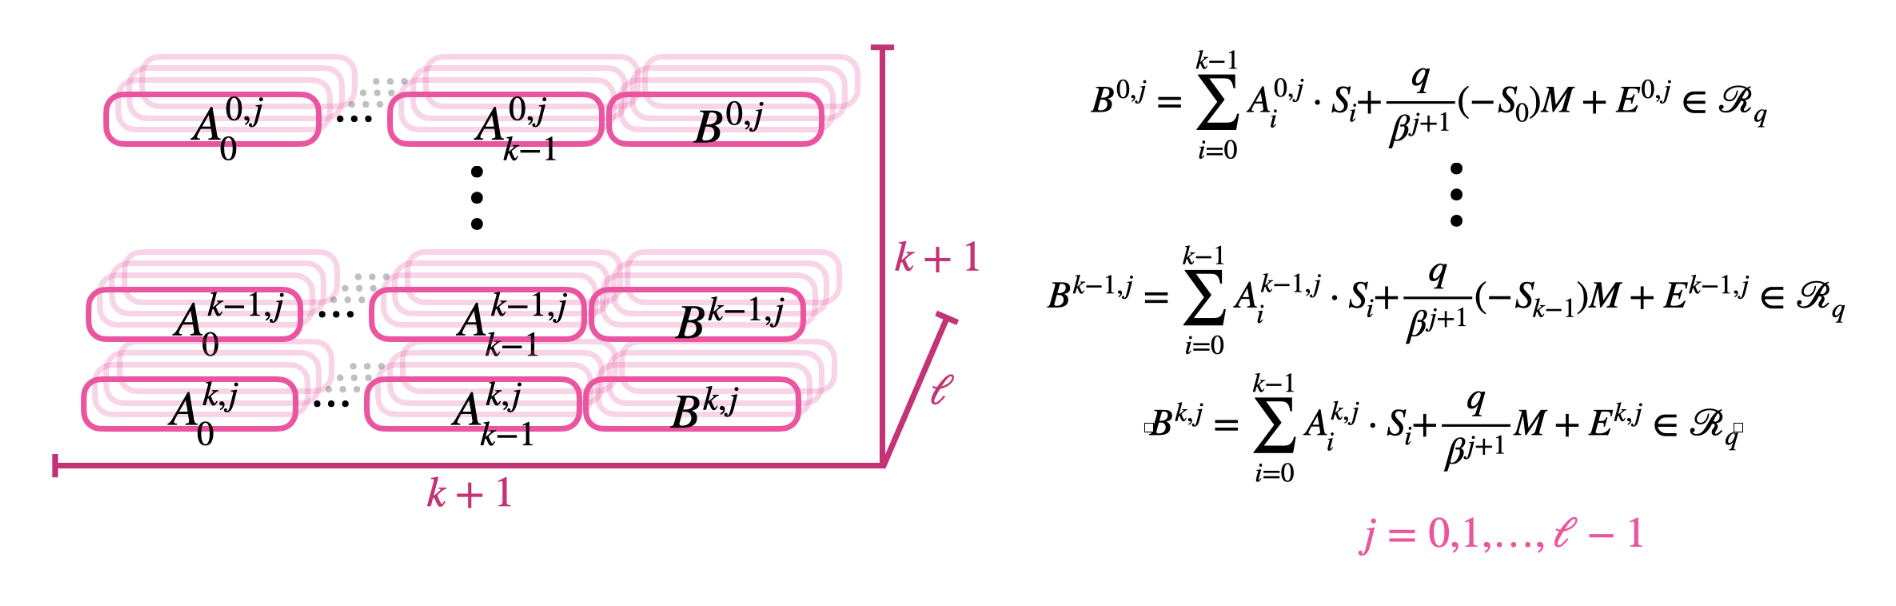
\includegraphics[width=.9\columnwidth]{fig/GGSW_1.png}
		\caption{GGSW}
		\label{fig:GGSW}
	\end{figure}

\subsection{GSW and RGSW from GGSW }
In the same way that we saw that GLWE was a generalization for both LWE and RLWE, we can observe that GGSW can be specialized into GSW and RGSW by following the same rules. When we instantiate GGSW with $k = n$ and $N = 1$, we get GSW.  When we instantiate GGSW with $k = 1$, we get RGSW.


\subsection{GLWE homomorphic addition}

A GLWE ciphertext encrypting the message M under the secret key $\overrightarrow{S}$ is a tuple:

	\begin{align*}
C = GLWE_{\overrightarrow{S},\sigma}(\bigtriangleup M)	&=	 (A_0,A_1,...A_{k-1}, B) \subseteq  R_{q}^{k+1} \\
	\end{align*}

Now, let’s consider another GLWE ciphertext encrypting the message $M^i$ under the same secret key

	\begin{align*}
C^i = GLWE_{\overrightarrow{S},\sigma}(\bigtriangleup M^i)	&=	 (A_0^i,A_1^i,...A_{k-1}^i, B^i) \subseteq  R_{q}^{k+1} \\
	\end{align*}

Then, we can add every component of the two ciphertexts and the result will be a new GLWE ciphertext encrypting the sum $M + M^i$ under the same secret key with noise that grew a little bit.

	\begin{align*}
C^+ = C+ C^i = GLWE_{\overrightarrow{S},\sigma}(\bigtriangleup M+M^i)	&=	 (A_0+A_0^i,A_1+A_1^i,...A_{k+1}+A_{k-1}^i, B+B^i) \subseteq  R_{q}^{k+1} \\
	\end{align*}

\subsection{GLWE homomorphic multiplication by a constant}
Let's now consider a small constant polynomial:

	\begin{align*}
		 \Lambda &=   \sum_{i=0}^{N-1}\Lambda_iX^i \in R  \\
	\end{align*}

Then, we can multiply the polynomial $\Lambda$ to every component of the ciphertext and the result will be a new GLWE ciphertext encrypting the product $\Lambda$. M under the same secret key with noise that grew a little bit 


	\begin{align*}
C^{(.)} = C.\Lambda = GLWE_{\overrightarrow{S},\sigma}(\bigtriangleup (\Lambda . M))	&=	 (\Lambda.A_0,\Lambda.A_1,...\Lambda.A_{k+1}, \Lambda.B) \subseteq  R_{q}^{k+1} \\
	\end{align*}

\subsection{Homomorphic multiplication by a large constant}
In GLWE homomorphic multiplication by a small constant polynomial, the noise grew proportionally concerning the size of the polynomial coefficients.
If we multiply every ciphertext component by a large constant $\beta$, the noise grows proportionally concerning its size and will compromise the result. 

\subsection{Decomposition and Inner products}
To solve the noise problem, we do decomposition and inner products. The idea involves decomposing the large constant into a small base $\beta$.

\begin{align*}
 \gamma &= \gamma_1\frac{q}{\beta^1} + \gamma_2\frac{q}{\beta^2} .... \gamma_l\frac{q}{\beta^l} 
 {Decomp}^{\beta l} 
\end{align*}

where where the decomposed elements ($\gamma_1, \gamma_2 ... \gamma_l$) are in $\Z_\beta$ and are small and both q and $\beta$ are power of 2.

\begin{align*}
 {Decomp}^{\beta l} = (\gamma_1, \gamma_2 ... \gamma_l)
\end{align*}

As the elements of the decomposition are small, we should now be able to perform multiplication with the ciphertext and have a negligible impact on the noise. But, to obtain as a result the product of $\gamma$ and the message M
 , we need to be able to invert the decomposition, and so to recompose $\gamma$
. To do that, instead of multiplying the decomposed elements by a GLWE encryption of M, we multiply them by the GLev encryption of M.

	\begin{figure}[H]
		\centering
	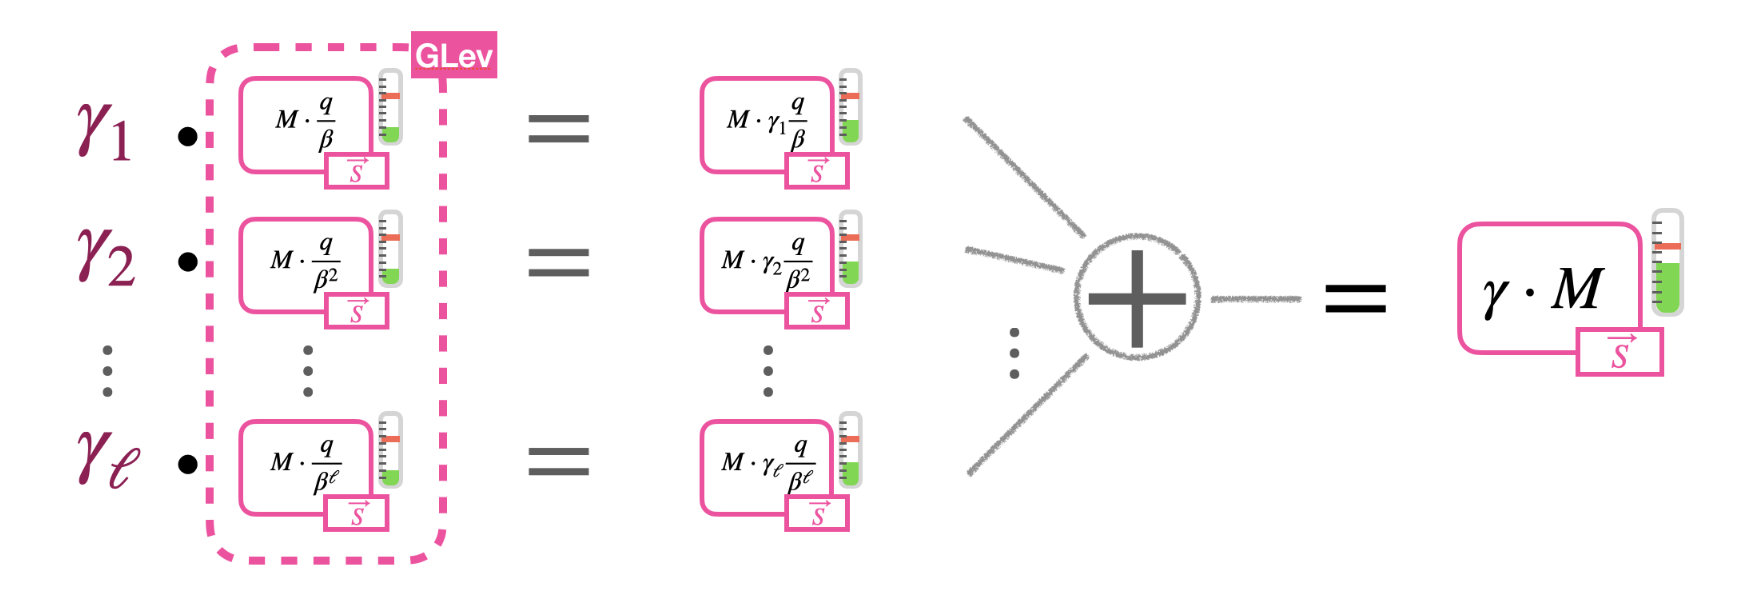
\includegraphics[width=.9\columnwidth]{fig/Glev_decomp.png}
		\caption{recompose using Glev}
		\label{fig:GLev_decomp}
	\end{figure}
 In this case, the noise grows very slowly since the multiplication times the small constants have a minor impact on the noise and the following addition.

\subsection{Homomorphic multiplication by a large polynomial}
Decompose the polynomial into small polynomials  and then perform a polynomial inner product with the GLev


\subsection{Approximate decomposition}

We could do an approximate decomposition and decompose to a fixed precision (using $\beta^l < q$). In practice, this means that we will do a rounding in the LSB part before decomposing: if the decomposition parameters are appropriately chosen, this will not affect the correctness of the computations because, in the LSB part, there is always noise and the information we are interested into keeping -- the message -- is in the MSB part. 

	\begin{figure}[H]
		\centering
	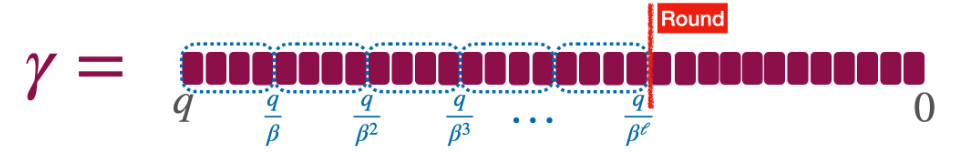
\includegraphics[width=.9\columnwidth]{fig/approx_decomp.png}
		\caption{Approximate decomposition}
		\label{fig:approx_decomp}
	\end{figure}

\subsubsection{Approximate decomposition example}
Let’s continue with previous examples for N (degree) = 4, p (plain modulus) = 4, k = 2, q = 64 (modulo) and $\bigtriangleup$ = q/p = 16.

Now let's choose a random large polynomial in $R_q$, so a polynomial of degree smaller than N = 4 and with coefficients in {-31, -30, ...-1, 0, 1, .. 32}:

	\begin{align*}
\Lambda	&=	 \Lambda_0 + \Lambda_1X^2 + \Lambda_2X^3 \\
                 &= 28 - 5X - 30X^2 + 17X^3 
	\end{align*}

Note that each coefficient consists of six bits.  -5 in signed decimal is 59 (64-5) unsigned decimal and (1,1,1,0,1,1) in binary. Similarly, -30 in signed decimal is 34 in unsigned decimal is $2^5 + 2^1$ (1,0,0,0,1,0) in binary.

Let's choose a base for the decomposition $\beta=4$ and l = 2, so $\beta^l=16$. Decomposed coefficients will be only 2 bits. We will decompose each coefficient's 4 MSB and round the last 2 LSB.

We need to round all the coefficients. First, we write them in their binary decomposition (MSB on the left and LSB on the right) and then round the LSB. 

	\begin{figure}[H]
		\centering
	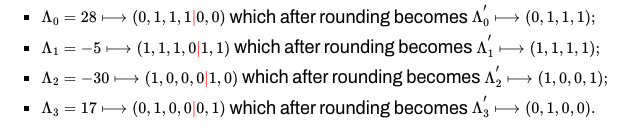
\includegraphics[width=.9\columnwidth]{fig/rounding.png}
		\caption{Rounding}
		\label{fig:rounding}
	\end{figure}

The next step is the decomposition. We start from the LSB and, since the base $\beta = 4$
We need to extract 2 bits for every round. We want the decomposition to be signed, so we want coefficients in {-2,-1,0,1}. So, in the binary decomposition, 

\begin{itemize}
  \item (0,0) corresponding to 0
  \item (0,1) corresponding to 1
  \item (1,0) corresponds to -2 (i.e. 2 - 4), and we add 4 to the next block in the decomposition, like a carry.
  \item (1,1) corresponds to -1 (i.e. 3 - 4), and we add 4 to the next block in the decomposition, like a carry.
\end{itemize}

Every carry that goes beyond the MSB is thrown away. 

	\begin{figure}[H]
		\centering
	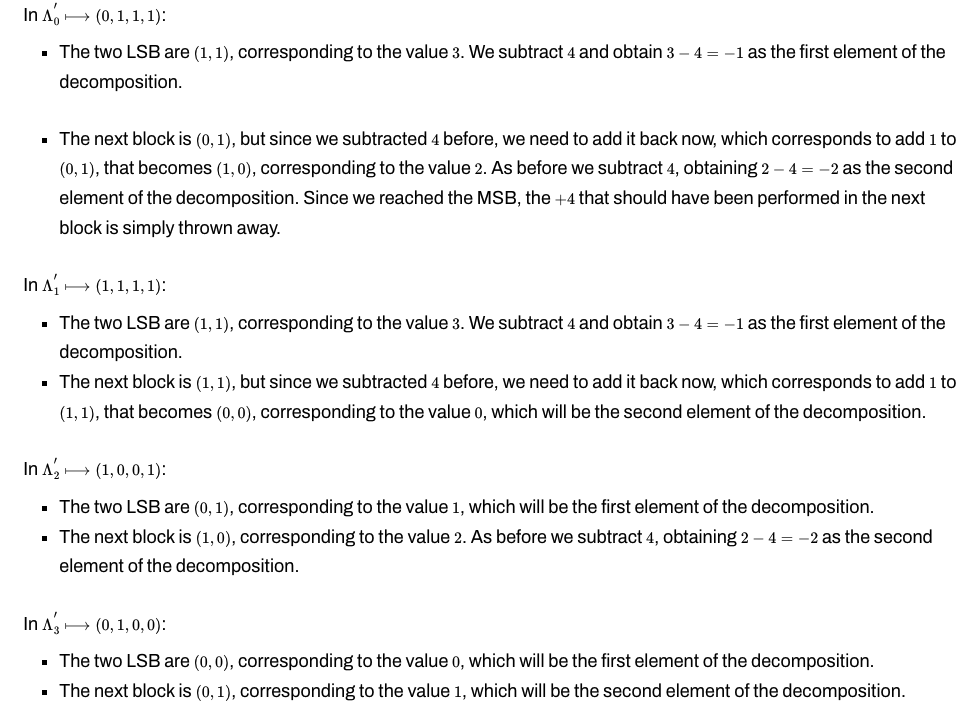
\includegraphics[width=1.1\columnwidth]{fig/lsb_rounding.png}
		\caption{decomposition of the coefficients}
		\label{fig:rounding_lsb}
	\end{figure}
Now that the decomposition of the coefficients is done, we can write explicitly the decomposed polynomials as:

	\begin{figure}[H]
		\centering
	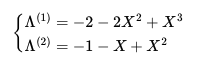
\includegraphics[width=.4\columnwidth]{fig/decomp_poly.png}
		\caption{Decomposed polynomial}
		\label{fig:decomposed_polyn}
	\end{figure}

The coefficients of $\Lambda^{(2)}$ are the first elements of the decomposition, while the coefficients of $\Lambda^{(1)}$ are the second elements of the decomposition. To verify that the decomposition is correct, we can invert it by computing:

	\begin{align*}
\Lambda^{(1)}.\frac{q}{\beta^1}	+ \Lambda^{(2)}.\frac{q}{\beta^2}	&=	  (-2-2X^2+X^3).\frac{64}{4^1}	+ (-1-X+X^2).\frac{64}{4^2} \\
 &= (-2-2X^2+X^3)16	+ (-1-X+X^2)4 \\
                 &= 28 - 5X - 28X^2+16X^3 \in R_{64}
	\end{align*}


\section{Key switching}
This homomorphic operation is primarily used in all the (Ring)LWE-based schemes. As the name suggests, it switches the secret key to a new one. To switch the key, we cancel the current secret key and homomorphically re-encrypt it under a new secret key. 

		\begin{align*}
{KSK}_i = (GLWE_{\overrightarrow{S^{'}},\sigma_{KSK}}(\frac{q}{\beta^1} S_i) \times ... \times GLWE_{\overrightarrow{S^{'}},\sigma_{KSK}}(\frac{q}{\beta^l} S_i))	&=	{GLev}_{\overrightarrow{S^{'}}, \sigma_{KSK}}^{\beta, l}(S_i)  \subseteq  R_{q}^{l{(k+1)}}  \\
	\end{align*}
	

The key switching is performed as follows:

	\begin{figure}[H]
		\centering
	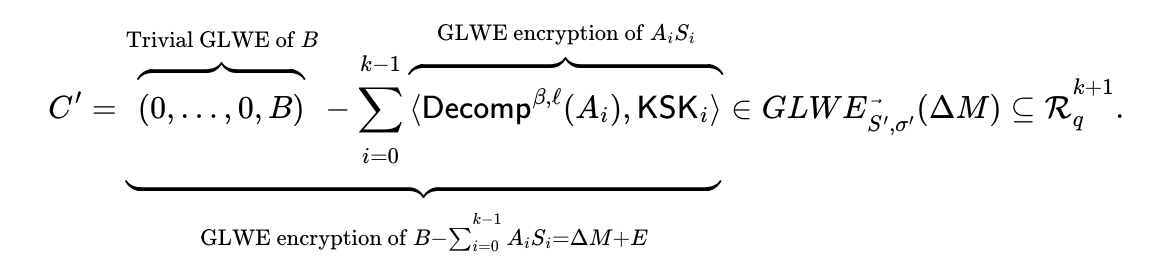
\includegraphics[width=1\columnwidth]{fig/ksk.png}
		\caption{Key switching}
		\label{fig:ksk}
	\end{figure}

The secret key has switched from $\overrightarrow{S}$ to $\overrightarrow{S^{'}}$, but the message is the same.

\end{document}
